% !Mode:: "TeX:UTF-8"
\chapter{Java基础}

\begin{introduction}
	\item 变量和类型
	\item 输入和输出
	\item 面向对象
	\item 异常处理
	\item 多线程
\end{introduction}

相比于其它编程语言,Java的语法不算多的,很容易掌握。
本章将以最短的篇幅带大家掌握Java编程语言。
编程语言三大核心要素:数据、语句和函数。
数据要先存放在变量中,才能被程序处理,不同类型的变量可存放不同的数据;
需要遍历所有的数据的时候,就会用到\lstinline{for/while}语句;
判断某个条件是否成立,使用\lstinline{if}语句等。
而把常用的逻辑放在一起,就定义了一个函数。

\section{jshell的使用}
本章部分内容,要在jshell(JDK9+)的交互式环境学习验证,请提前配置环境变量。
你可在单台机器上安装多个JDK版本\footnote{DeepLearning4i需要JDK8。},
只要确保你的配置是正确的,就没有关系。

\begin{lstlisting}[language=bash]
	jshell> /help
|  键入 Java 语言表达式, 语句或声明。
|  或者键入以下命令之一:
|  /list [<名称或 id>|-all|-start]
|  	列出您键入的源
|  /save [-all|-history|-start] <文件>
|  	将片段源保存到文件
|  /open <file>
|  	打开文件作为源输入
|  /vars [<名称或 id>|-all|-start]
|  	列出已声明变量及其值
|  /methods [<名称或 id>|-all|-start]
|  	列出已声明方法及其签名
|  /types [<名称或 id>|-all|-start]
|  	列出类型声明
|  /imports 
|  	列出导入的项
|  /exit [<integer-expression-snippet>]
|  	退出 jshell 工具
\end{lstlisting}

使用jshell可以快速验证我们的代码是否正确,并支持类型推断(var)。
下面2个变量定虽然没有设定类型,但根据下一节介绍的规则,可自动推理为int和double类型:
\begin{lstlisting}[language=bash, backgroundcolor=\color{lightgray!10}]
	jshell> var m = 2
	m ==> 2
	jshell> var n = 3.0
	n ==> 3.0
	jshell> /vars
	|    int m = 2
	|    double n = 3.0
\end{lstlisting}

\section{变量和类型}
与其他静态类型语言一样,java支持的基本数据类型有:
\lstinline{byte、char、short、int、long、float、double}
等。

\begin{table}[!htbp] \centering \small
\begin{tabular}{|p{1cm}|p{3cm}|p{9cm}|}
\toprule
	\multicolumn{3}{|c|}{基本类型 - 范围}\\
\midrule
	byte&8位(一个字节)&$-128\sim127$\\
	short&16位(两个字节)&$-32768\sim32767$\\
	char&16位(两个字节)&$-32768\sim32767$\\
	int&32位(四个字节)&$-2147483648\sim2147483647$\\
	long&64位(八个字节)&$-9223372036854774808\sim9223372036854775807$\\
	float&32位(四个字节)&$1.401298e-45\sim3.402823e+38$\\
	double&64位(八个字节)&$4.9000000e-324\sim1.797693e+308$\\
\bottomrule
\end{tabular}
	\caption{基本数据类型}
\end{table}

基本类型的数值范围,可在相应的封装类型中获得。
譬如\lstinline{int}的封装类型是Integer,称为装箱,反之称为拆箱。
\begin{enumerate}
	\item byte -> Byte
	\item short-> Short
	\item int -> Integer
	\item long -> Long
	\item float -> Float
	\item double -> Double
\end{enumerate}

\begin{lstlisting}[language=Java, backgroundcolor=\color{lightgray!10}]
	jshell> Long.M   // 按TAB键,可自动补全
	MAX_VALUE   MIN_VALUE   
	jshell> Long.MAX_VALUE
	$15 ==> 9223372036854775807
	jshell> Double.MAX_VALUE
	$16 ==> 1.7976931348623157E308
	jshell> Double.MIN_VALUE
	$17 ==> 4.9E-324
\end{lstlisting}

\begin{definition}{变量}{var}
	$[\text{类型}]$ 变量名称, 变量名称 $=$ 初值, $\dots$;\\
	$[\text{类型}]$ 变量名称 $=$ 初值;
\end{definition}

\begin{lstlisting}[language=java]
	int n1, n2=2, n3;
	float f1 = 0.2f;
\end{lstlisting}

\remark{
	变量要在初始化之后,才能使用。代码中小数默认是double类型,需要加后缀f才代表float。
}

\bigskip
当数据与类型不一致时,就会发生数据类型转换。
Java语言提供从小范围到大范围的自动转换,但反过来必须显式强制转换。

\begin{lstlisting}[language=java]
	byte b = 100; // 超过127会提示错误!编译器识别为int
	int n = b;
	float f = 0.2f;
	double d = f;

	int n2 = 100;
	byte b2 = (byte)n2
	double d2 = 0.2; // 小数默认是double类型
	float f2 = (float)d2;
\end{lstlisting}

\bigskip

\begin{exercise}
	把int类型的值强制赋值给byte变量,会出现什么问题?
\end{exercise}

\begin{exercise}
	把byte=-1赋值给int类型变量,该变量的值是多少?
\end{exercise}

\begin{exercise}
	已知byte=-1原本是正整数赋值得到的,如何再赋值给int类型变量,该正数是多少呢?
\end{exercise}

\subsection{数组}
表示很多个某一类数据的时候,就要用到数组,譬如某地区的房价。
通过下标使用数组中的值,第一个下标为0,依次往后递增,最后一个下标是length-1。
Java数组下标只能是整数,不支持字符串等其他类型。
房价数据保留小数点后2-3位精度就足够了,定义float类型数组如下:

\begin{definition}{数组}{array}
	$[\text{类型}]\quad[]$变量名称;\\
	$[\text{类型}]\quad[]$变量名称 = \{131.2, 110.8, 117.34\};\\
	$[\text{类型}]\quad[]$变量名称 = new 类型$[$总数$]$\};\\
	$[\text{类型}]\quad[]$变量名称 = new 类型$[]$\{131.2, 110.8\};
\end{definition}

\begin{lstlisting}[language=java]
	float []prices = {131.2, 110.8, 117.34};
	float []areas = new float[]{90, 120, 114};
\end{lstlisting}

\remark{
	byte数组内容,不能赋值给int类型的数组,强制转换也不行。
}
\bigskip

以上称之为一位数组。
若提供的房价数据,不止一个地区的,就需要二维数组表示:
houses[地区][下标]。
若需要创建更多维度的数组,以此类推:
patients[性别][年龄][下标]可定位某个病人的状态。
Java数组不要求每一行的长度相等,譬如30岁女性的病人有17个而34岁女性的病人可能是2个或者0个。

\begin{lstlisting}[language=java]
	float [][]houses = {
				{131.2f, 110.8f, 91.09f},
				{157.8f, 107.13f, 105.71f},
				{98.4f, 119.54f, 117.44f},
	};
	int area = 1, index = 2; // 第2地区,第3处房子的价格
	float price23 = prices[area][index];
	System.out.printf("%f", price23); // 输出105.709999
\end{lstlisting}

\remark{
	浮点类型:float和double不是准确数字,只能保证精度。
	因此不要直接和某个浮点数比较是否相等,在允许范围内即可。
}
\bigskip

\begin{example}
	波士顿房价数据集(Boston House Price Dataset)
	,该数据集是美国人口普查局收集的有关波士顿马萨诸塞州住房的信息,发表于1978年美国某经济学杂志。
	该数据集包含波士顿房屋的价格及其各项数据,每个数据项有14个数据,常用于回归分析。
	数据集中包含506组数据,其中404是训练样本,剩下的102组数据作为验证样本。
	\bigskip

	\begin{table}[!htbp]\centering \scriptsize
    \csvautobooktabular{part1/boston-sample.csv}
	\end{table}

	\begin{itemize} \small
		\item CRIM    - 城镇人均犯罪率。
		\item ZN      - 占地面积超过25,000平方英尺的住宅用地比例。
		\item INDUS   - 城镇非零售商用土地的比例。
		\item CHAS    - Charles River虚拟变量(如果是河道,则为1;否则为0)。
		\item NOX     - 一氧化氮浓度(每千万)
		\item RM      - 每栋住宅的房间数。
		\item AGE     - 1940年之前建成的自用房屋比例。
		\item DIS     - 到波士顿五个中心区域的加权距离。
		\item RAD     - 径向高速公路的可达性指数。
		\item TAX       - 每10,000美元的全额物业税率。
		\item PTRATIO - 城镇的学生与教师比例。
		\item B       - $1000(Bk - 0.63)^ 2$,其中Bk是城镇黑人的比例。
		\item LSTAT   - 人口中地位低下者的比例。
		\item MEDV    - 自住房屋房价中位数(也就是均价)。
	\end{itemize}
	\medskip \noindent
	借助Excel把散点图绘制出来,可直观发现各因素与房价的关系。
	其中,RM就和MDEV就明显存在强线性关系,毕竟房子越大房价就会越贵。
	现在我们用Java数组把RM、MEDV列所有数据表示出来。
	\begin{lstlisting}[language=java]
	double []RM = {6.575, 6.421, 7.185, 6.998, 7.147, 6.43, 6.012, 6.172, 5.631};
	double []MDEV = {24, 21.6, 34.7, 33.4, 36.2, 28.7, 22.9, 27.1, 16.5};
	\end{lstlisting}

	\begin{figure}[!htb]
		\centerline{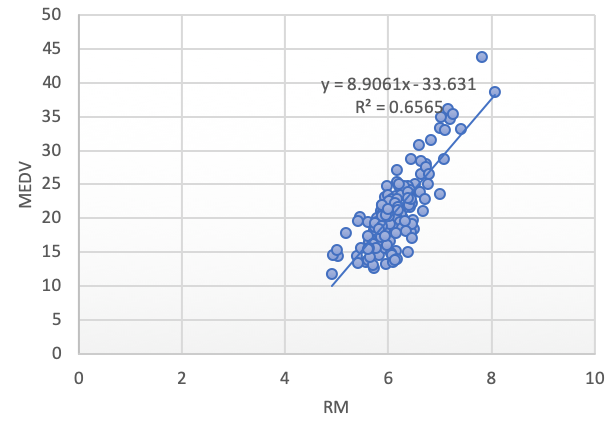
\includegraphics{part1/boston-rm.png}}
	\end{figure}
\end{example}


\begin{exercise}
	double类型的精度是多少?
\end{exercise}

\begin{exercise}
	检查是否与3.14相等的代码?
\end{exercise}

\section{字典}


\section{语句}

\section{函数}